
\section{Planning Language}\label{S:PDDL}
The Planning Domain Definition Language (PDDL) \cite{PDDL} is an attempt by the domain independent planning community to formulate a standard language for planning. A community of planning researchers has been producing planning systems that comply with this formalism since the first International Planning Competition held in 1998. This competition series
continues today, with the seventh competition being held in 2011. PDDL is constantly adding extensions to the base language in order to represent more expressive problem domains. Our work is based on PDDL Version 3.\\
By placing our knowledge in a PDDL representation, we enable the use of an entire family of open source planning systems.
Each PDDL file-set consists of two files that specify the domain and the problem.

\subsection{The PDDL Domain File}\label{S:PDDL-domain}
The PDDL domain file for kitting is consists of five sections that include \texttt{requirements}, \texttt{types}, \texttt{predicates}, \texttt{functions}, and \texttt{actions}. An excerpt of the PDDL domain file is depicted in Figure~\ref{fig:domain}.

\begin{figure}[t!h!]
\begin{minipage}{.5\paperwidth}
\begin{mylisting}
\begin{Verbatim}[commandchars=\\\{\},fontsize=\scriptsize, numbers=left, numbersep=2pt]
(define (domain kitting-domain)
    (:requirements :strips :typing :fluents)
    (:types EndEffector EndEffectorHolder Kit KitTray LargeBoxWithEmptyKitTrays 
        PartsTray EndEffectorChangingStation Robot WorkTable LargeBoxWithKits Part)

    (:predicates
	   (endeffector-location-robot ?endeffector - EndEffector ?robot - Robot)	
	   (on-worktable-kit ?worktable - WorkTable ?kit - Kit))

    (:functions
	   (quantity-partstray ?partstray - PartsTray)
	   (quantity-kit ?kit - Kit ?partstray - PartsTray)
	   (capacity-kit ?kit - Kit ?partstray - PartsTray))

    (:action take-kittray
        :parameters(
            ?robot - Robot
            ?kittray - KitTray
            ?largeboxwithemptykittrays - LargeBoxWithEmptyKitTrays
            ?endeffector - EndEffector
            ?worktable - WorkTable)
        :precondition(and
            (robot-empty ?robot)
            (lbwekt-not-empty ?largeboxwithemptykittrays)
            (robot-with-endeffector ?robot ?endeffector)
            (kittray-location-lbwekt ?kittray ?largeboxwithemptykittrays)
            (endeffector-location-robot ?endeffector ?robot)
            (worktable-empty ?worktable)
            (endeffector-type-kittray ?endeffector ?kittray))
        :effect(and
            (robot-holds-kittray ?robot ?kittray)
            (kittray-location-robot ?kittray ?robot)
            (not (robot-empty ?robot))
            (not (kittray-location-lbwekt ?kittray ?largeboxwithemptykittrays))))
)

\end{Verbatim}
\end{mylisting}
\end{minipage}
\caption{Excerpt of the PDDL domain file for kitting.}
\label{fig:domain}
\end{figure}

\begin{itemize}
\item line 1: The keyword \texttt{domain} signals a planner that this file contains information on the domain. \texttt{kitting-domain} is the name given to the domain.
\item line 2: The \texttt{:requirements} field specifies which section the domain relies on. The planning system can examine this statement to determine if it is capable of solving problems in this domain. A keyword (symbol starting with a colon) used in a \texttt{:requirements} field is called a requirement flag; the domain is said to declare a requirement for that flag. The requirement flags present in the kitting domain are:
\begin{itemize}
\item \texttt{:strips}: The most basic subset of PDDL, consisting of STRIPS only.
\item \texttt{:typing}: PDDL has a special syntax for declaring parameter and object types. \texttt{:typing} allows types names in declaration of variables.
\item \texttt{:fluents}: A domain's set of requirements allow a planner to quickly tell if it is likely to be able
to handle the domain. For example, this version of the kitting world requires fluents numeric, so a straight STRIPS-representation planner would not be able to handle it. A fluent is a term (\texttt{:functions}) with time-varying value (i.e., a value that can change as a result of performing an action).
\end{itemize}
\item lines 3--4:  Type names have to be declared before they are used (before \texttt{:predicates} and \texttt{:functions}). This is done with the declaration \texttt{(:types $name_1$ ... $name_n$)}.
\item lines 6--8: The \texttt{:predicates} part of a domain definition specify only what are the predicate names used in the domain, and their number of arguments (and argument types, if the domain uses \texttt{:typing}). The ``meaning'' of a predicate, in the sense of for what combinations of arguments it can be true and its relationship to other predicates, is determined by the effects that actions in the domain can have on the predicate, and by what instances of the predicate are listed as true in the initial state of the problem definition.\\
    It is common to make a distinction between static and dynamic predicates. A \textit{static} predicate is not changed by any action. Thus in a problem, the true and false instances of a \textit{static} predicate will always be precisely those listed in the initial state specification of the problem definition. Note that there is no syntactic difference between \textit{static} and \textit{dynamic} predicates in PDDL, they look exactly the same in the \texttt{:predicates} declaration part of the domain.\\
    A predicate is build using the structure \texttt{(predicate\_name ?X - type\_of\_X)}. A list of parameters of the same type in a predicate can be abbreviated to \texttt{(predicate\_name ?X ?Y ?Z - type\_of\_XYZ)}. Note that the hyphen between parameter and type name is surrounded by whitespace.
\item lines 10--13: A fluent is similar to a state variable/predicate except that its value is a number instead of true or false. The initial value of a function is set in the initial state of the problem file and changes when an action is executed. The declaration of functions is similar to predicates.
\item lines 15--34: The domain definition contains operators (called \textit{actions} in PDDL). An action statement specifies a way that a planner affects the state of the world. The statement includes parameters, preconditions, and effects. All parts of an action definition except the name are, according to the PDDL specification, optional (although, of course, an action without effects is pretty useless). However, for an action that has no preconditions some planners may require an ``empty'' precondition, on the form :precondition () or :precondition (and), and some planners may also require an empty :parameter list for actions without parameters).
\begin{itemize}
\item lines 16--21: The \texttt{:parameters} section declare all the parameters used by predicates and functions in \texttt{preconditions} and \texttt{effects}.
\item lines 22--29: The \texttt{:preconditions} section is a conjunction of predicates and functions that need to be true in the world in order for the action to be invoked.
\item lines 30--34: The \texttt{:effects} equation dictates the changes in the world that will occur due to the execution of the action.
\end{itemize}
\end{itemize}


\subsection{PDDL Problem File}\label{S:PDDL-problem}
The second file of the PDDL file-set is a  problem file. The problem file specifies information about the specific instance of the given problem. This file contains the initial conditions and definition of the world (in the \texttt{init} section) and the final state that the world must be brought to (in the \texttt{goal} section). Using an example of kit to build, this section only describes the initial and goal states explicitly. The operators detailed in Section~\ref{subsect:Planning_Operators} are used by a planner to generate the other states as needed.\\
In the PDDL problem file depicted below, the \class{Robot} has to build a kit that contains two \class{Parts} of type A, one \class{Part} of type B and one \class{Part} of type C. The kitting process is completed once the \class{Kit} is placed in the \class{LargeBoxWithKits}.

\begin{center}
\begin{minipage}{.9\paperwidth}
\begin{mylisting}
\begin{Verbatim}[commandchars=\\\{\},fontsize=\scriptsize, numbers=left, numbersep=2pt]
(define (problem kitting-problem)
    (:domain kitting-domain)
    (:objects
        robot_1 - Robot
        changing_station_1 - EndEffectorChangingStation
        kit_tray_1 - KitTray
        kit_a2b1c1 - Kit
        empty_kit_tray_supply - LargeBoxWithEmptyKitTrays
        finished_kit_receiver - LargeBoxWithKits
        work_table_1 - WorkTable
        part_a_tray part_b_tray part_c_tray - PartsTray
        part_a_1 part_a_2  - Part
        part_b_1 part_b_2 part_b_3 - Part
        part_c_1 part_c_2 - Part
        part_gripper tray_gripper - EndEffector
        part_gripper_holder tray_gripper_holder - EndEffectorHolder
    )
)
(:init
    (robot-with-no-endeffector robot_1)
    (part-not-searched)
    (lbwekt-not-empty empty_kit_tray_supply)	
    (lbwk-not-full finished_kit_receiver)		
    (partstray-not-empty part_a_tray)
    (partstray-not-empty part_b_tray)
    (partstray-not-empty part_c_tray)
    (endeffector-location-endeffectorholder part_gripper part_gripper_holder)
    (endeffector-location-endeffectorholder tray_gripper tray_gripper_holder)
    (endeffectorholder-holds-endeffector part_gripper_holder part_gripper)
    (endeffectorholder-holds-endeffector tray_gripper_holder tray_gripper)
    (endeffectorholder-location tray_gripper_holder changing_station_1)
    (endeffectorholder-location part_gripper_holder changing_station_1)
    (endeffectorchangingstation-contains-endeffectorholder changing_station_1 tray_gripper_holder)	
    (endeffectorchangingstation-contains-endeffectorholder changing_station_1 part_gripper_holder)
    (worktable-empty work_table_1)
    (kittray-location-lbwekt kit_tray_1 empty_kit_tray_supply)

\end{Verbatim}
\end{mylisting}
\end{minipage}

\begin{minipage}{.5\paperwidth}
\begin{mylisting}
\begin{Verbatim}[commandchars=\\\{\},fontsize=\scriptsize,  firstnumber=continue, numbers=left, numbersep=2pt]	

    (part-location-partstray part_a_1 part_a_tray)
    (part-location-partstray part_a_2 part_a_tray)
    (part-location-partstray part_b_1 part_b_tray)
    (part-location-partstray part_b_2 part_b_tray)
    (part-location-partstray part_b_3 part_b_tray)
    (part-location-partstray part_c_1 part_c_tray)
    (part-location-partstray part_c_2 part_c_tray)
	
    (endeffector-type-part part_gripper part_a_1)
    (endeffector-type-part part_gripper part_a_2)
    (endeffector-type-part part_gripper part_b_1)
    (endeffector-type-part part_gripper part_b_2)
    (endeffector-type-part part_gripper part_b_3)
    (endeffector-type-part part_gripper part_c_1)
    (endeffector-type-part part_gripper part_c_2)

    (endeffector-type-kittray tray_gripper kit_tray_1)
    (endeffector-type-kit tray_gripper kit_a2b1c1)

    (= (capacity-kit kit_a2b1c1 part_a_tray) 2)
    (= (capacity-kit kit_a2b1c1 part_b_tray) 1)
    (= (capacity-kit kit_a2b1c1 part_c_tray) 1)

    (= (quantity-kit kit_a2b1c1 part_a_tray) 0)
    (= (quantity-kit kit_a2b1c1 part_b_tray) 0)
    (= (quantity-kit kit_a2b1c1 part_c_tray) 0)
\end{Verbatim}
\end{mylisting}
\end{minipage}

\begin{minipage}{.5\paperwidth}
\begin{mylisting}
\begin{Verbatim}[commandchars=\\\{\},fontsize=\scriptsize,  firstnumber=continue, numbers=left, numbersep=2pt]	
    (= (quantity-partstray part_a_tray) 2)
    (= (quantity-partstray part_b_tray) 3)
    (= (quantity-partstray part_c_tray) 2)

    (origin-part part_a_1 part_a_tray)
    (origin-part part_a_2 part_a_tray)
    (origin-part part_b_1 part_b_tray)
    (origin-part part_b_2 part_b_tray)
    (origin-part part_b_3 part_b_tray)
    (origin-part part_c_1 part_c_tray)
    (origin-part part_c_2 part_c_tray)
)

(:goal
    (and
        (= (quantity-kit kit_a2b1c1 part_a_tray)(capacity-kit kit_a2b1c1 part_a_tray))
        (= (quantity-kit kit_a2b1c1 part_b_tray)(capacity-kit kit_a2b1c1 part_b_tray))
        (= (quantity-kit kit_a2b1c1 part_c_tray)(capacity-kit kit_a2b1c1 part_c_tray))
        (kit-location-lbwk kit_a2b2c1 finished_kit_receiver)
    )
)
\end{Verbatim}
\end{mylisting}
\end{minipage}
\end{center}

\begin{itemize}
\item line 1: Signal a planner that the file contains all the element part of a problem. \texttt{kitting-problem} is the name given to this problem.
\item line 2: \texttt{:domain} refers to the domain that the current problem is associated to. In this case, the problem refers to the domain \texttt{kitting-domain}. Note that \texttt{kitting-domain} is the name given to the kitting domain as presented in section~\ref{S:PDDL-domain}.
\item line 3--17: \texttt{:objects} declare objects present in the problem instance. The syntax for \texttt{:objects} is \texttt{$object_1$ - Type ... $object_n$ - Type}.
\end{itemize}
%\caption{The init section.}
%\label{fig:init}
%\end{figure}

\subsubsection{Initial State}
The initial state $S_0$ (Figure~\ref{fig:s0}) defines the environment in its initial condition. The initial state of the kitting problem in PDDL format is described below.

\begin{figure}[h!t!]
\centering
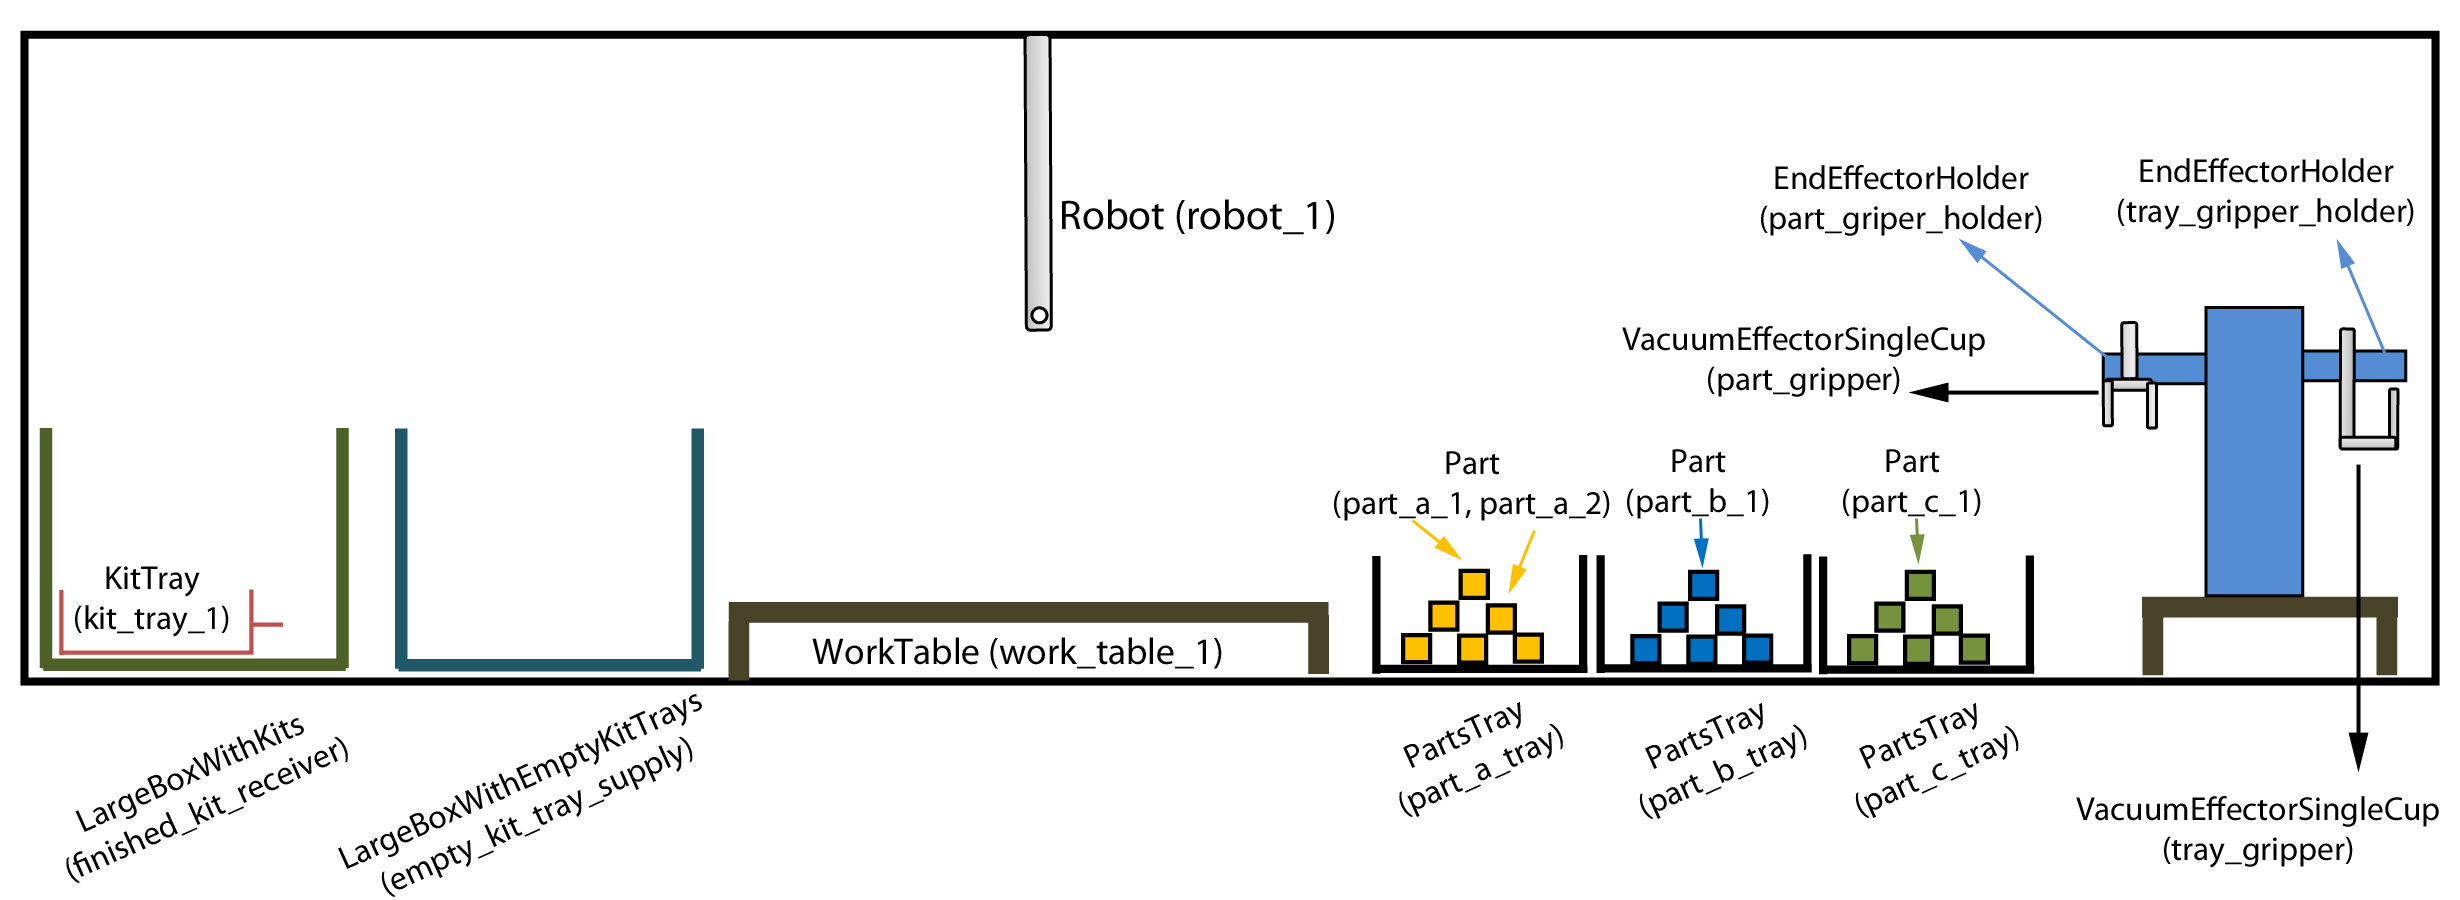
\includegraphics[width=14cm]{Figure/s0.jpg}
\caption{Initial state $S_0$.}
\label{fig:s0}
\end{figure}

\begin{itemize}
\item line 19: \texttt{:init} signals a planner that the predicates and functions in this section are true in the initial state.
\item line 20--76: Predicates true in the initial state of the environment. Since PDDL uses a close world assumption, predicates that are not present in the initial state are automatically set to false. This section also set the initial values for functions. Some relevant sections are presented:
\begin{itemize}
\item line 21: The predicate \stvarsmall{part-not-searched} is set to true so that the operator \op{look-for-part} can be activated during a plan search.
\item line 58--60: Functions describing how many parts of a specific type that \constsmall{kit\_a2b1c1} can contain. In this example, \constsmall{kit\_a2b1c1} can have two \class{Parts} of type A (\constsmall{part\_a\_tray}), one \class{Part} of type B (\constsmall{part\_b\_tray}), and one \class{Part} of type C (\constsmall{part\_c\_tray}).
\item line 62--64: Functions that represent the number of parts of a specific type that are already in \constsmall{kit\_a2b1c1}. In the initial state, \constsmall{kit\_a2b1c1} is empty (no \class{Parts} of type A, B, or C).
\item line 65--67: Functions that describe the number of parts available in their respective parts tray. This also can be read as: \emph{In the workstation, there are two \class{Parts} of type A available, three \class{Parts} of type B available, and three \class{Parts} of type C available}.
\item line 69--75: Predicates that describe the type of each specific part in the workstation. Defining that \texttt{part\_a\_1} is from \texttt{part\_a\_tray} is similar to \texttt{part\_a\_tray} is of type A since a \class{PartsTray} consists of parts of the same type.
\end{itemize}
\end{itemize}

\subsubsection{Goal State}
\begin{figure}[h!t!]
\centering
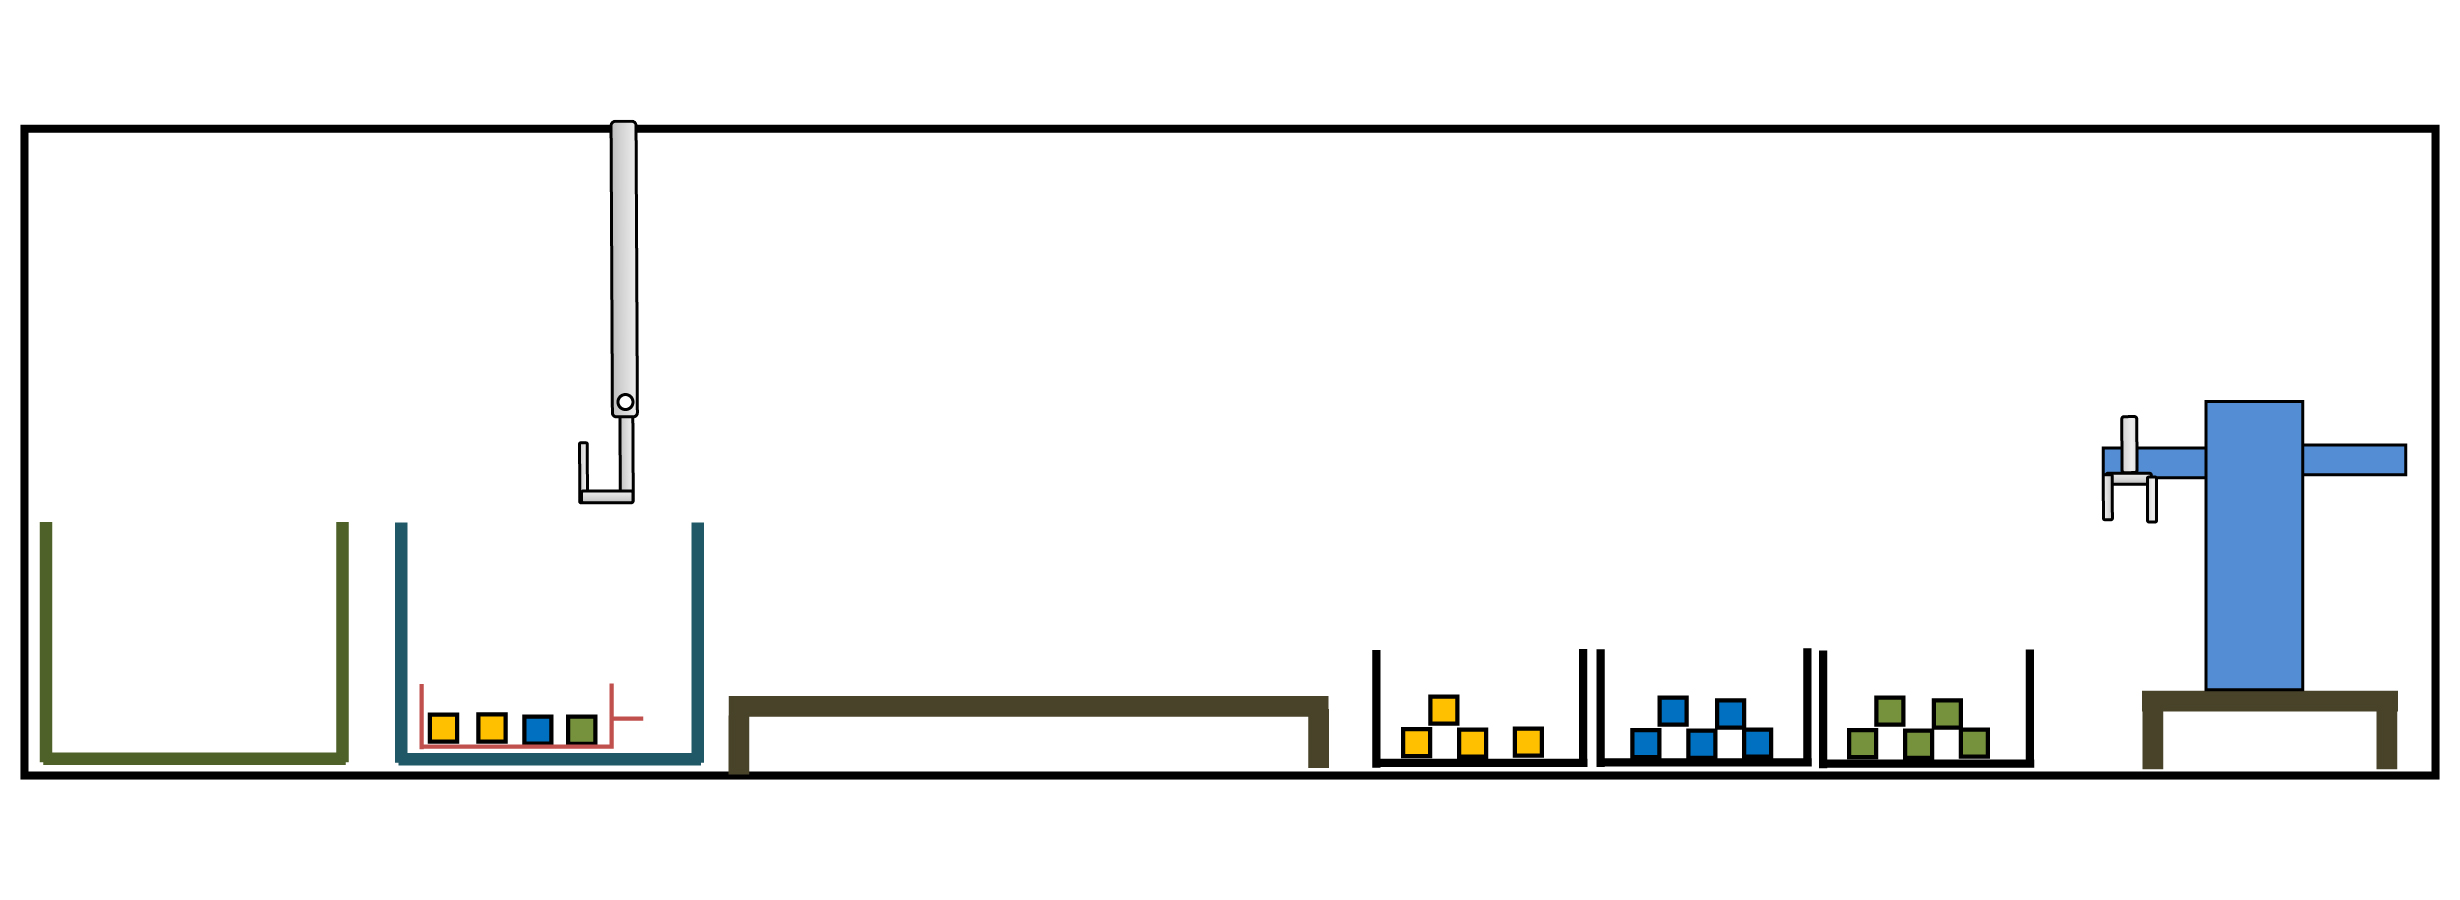
\includegraphics[width=14cm]{Figure/sfinal.jpg}
\caption{Goal state $S_G$.}
\label{fig:sf}
\end{figure}
Figure~\ref{fig:sf} depicts the goal state $S_G$ for the kitting workstation. The expression of the goal state in PDDL is described below.


\begin{itemize}
\item line 78: \texttt{:goal} is a keyword used to signal a planner about the goal state to reach. All the predicates and functions in the goal state must be true.
\item line 80--82: The quantity of parts of a specific type in \constsmall{kit\_a2b1c1} should match the capacity of parts of a specific type for \constsmall{kit\_a2b1c1}. The quantity of parts in \constsmall{kit\_a2b1c1} is increased in the operator \op{put-part}. The initial quantity of parts in \constsmall{kit\_a2b1c1} (lines 62--64) and its capacity (lines 58--60) are set in the initial state. Note that we are not specifying which instance of \class{Part} should go in \constsmall{kit\_a2b1c1} but rather the number of \class{Parts} of a specific type that \constsmall{kit\_a2b1c1} must have.
\item line 83: \constsmall{kit\_a2b1c1} should be placed in the large box with kits \constsmall{finished\_kit\_receiver}.
\end{itemize}

\subsection{Plan}
This section shows an example of a plan generated by a planner (see section~\ref{section:planner}) for the PDDL domain and problem files discussed previously in this document.

 Figure~\ref{fig:plan} displays the different states and actions used by the planner to generate a plan starting from the initial state $S_0$ to the goal state $S_G$. The actions $A_1$ \ldots $A_{17}$ are described below.
\begin{itemize}
\item $A1$:(\opsmall{attach-endeffector} \constsmall{robot\_1} \constsmall{tray\_gripper} \constsmall{tray\_gripper\_holder} \constsmall{changing\_station\_1})
\item $A2$:(\opsmall{take-kittray} \constsmall{robot\_1} \constsmall{kit\_tray\_1} \constsmall{empty\_kit\_tray\_supply} \constsmall{tray\_gripper} \constsmall{work\_table\_1})
\item $A3$:(\opsmall{put-kittray} \constsmall{robot\_1} \constsmall{kit\_tray\_1} \constsmall{work\_table\_1})
\item $A4$:(\opsmall{create-kit} \constsmall{kit\_a2b2c1} \constsmall{kit\_tray\_1} \constsmall{work\_table\_1})
\item $A5$:(\opsmall{remove-endeffector} \constsmall{robot\_1} \constsmall{tray\_gripper} \constsmall{tray\_gripper\_holder} \constsmall{changing\_station\_1})
\item $A6$:(\opsmall{attach-endeffector} \constsmall{robot\_1} \constsmall{part\_gripper} \constsmall{part\_gripper\_holder} \constsmall{changing\_station\_1})
\item $A7$:(\opsmall{look-for-part} \constsmall{robot\_1} \constsmall{part\_c\_1} \constsmall{part\_c\_tray} \constsmall{kit\_a2b2c1} \constsmall{work\_table\_1} \constsmall{part\_gripper})
\item $A8$:(\opsmall{take-part} \constsmall{robot\_1} \constsmall{part\_c\_1} \constsmall{part\_c\_tray} \constsmall{part\_gripper} \constsmall{work\_table\_1} \constsmall{kit\_a2b2c1})
\item $A9$:(\opsmall{put-part} \constsmall{robot\_1} \constsmall{part\_c\_1} \constsmall{kit\_a2b2c1} \constsmall{work\_table\_1} \constsmall{part\_c\_tray})
\item $A10$:(\opsmall{look-for-part} \constsmall{robot\_1} \constsmall{part\_b\_2} \constsmall{part\_b\_tray} \constsmall{kit\_a2b2c1} \constsmall{work\_table\_1} \constsmall{part\_gripper})
\item $A11$:(\opsmall{take-part} \constsmall{robot\_1} \constsmall{part\_b\_2} \constsmall{part\_b\_tray} \constsmall{part\_gripper} \constsmall{work\_table\_1} \constsmall{kit\_a2b2c1})
\item $A12$:(\opsmall{put-part} \constsmall{robot\_1} \constsmall{part\_b\_2} \constsmall{kit\_a2b2c1} \constsmall{work\_table\_1} \constsmall{part\_b\_tray})
\item $A13$:(\opsmall{look-for-part} \constsmall{robot\_1} \constsmall{part\_b\_1} \constsmall{part\_b\_tray} \constsmall{kit\_a2b2c1} \constsmall{work\_table\_1} \constsmall{part\_gripper})
\item $A14$:(\opsmall{take-part} \constsmall{robot\_1} \constsmall{part\_b\_1} \constsmall{part\_b\_tray} \constsmall{part\_gripper} \constsmall{work\_table\_1} \constsmall{kit\_a2b2c1})
\item $A15$:(\opsmall{put-part} \constsmall{robot\_1} \constsmall{part\_b\_1} \constsmall{kit\_a2b2c1} \constsmall{work\_table\_1} \constsmall{part\_b\_tray})
\item $A16$:(\opsmall{look-for-part} \constsmall{robot\_1} \constsmall{part\_a\_2} \constsmall{part\_a\_tray} \constsmall{kit\_a2b2c1} \constsmall{work\_table\_1} \constsmall{part\_gripper})
\item $A17$:(\opsmall{take-part} \constsmall{robot\_1} \constsmall{part\_a\_2} \constsmall{part\_a\_tray} \constsmall{part\_gripper} \constsmall{work\_table\_1} \constsmall{kit\_a2b2c1})
\item $A18$:(\opsmall{put-part} \constsmall{robot\_1} \constsmall{part\_a\_2} \constsmall{kit\_a2b2c1} \constsmall{work\_table\_1} \constsmall{part\_a\_tray})
\item $A19$:(\opsmall{look-for-part} \constsmall{robot\_1} \constsmall{part\_a\_1} \constsmall{part\_a\_tray} \constsmall{kit\_a2b2c1} \constsmall{work\_table\_1} \constsmall{part\_gripper})
\item $A20$:(\opsmall{take-part} \constsmall{robot\_1} \constsmall{part\_a\_1} \constsmall{part\_a\_tray} \constsmall{part\_gripper} \constsmall{work\_table\_1} \constsmall{kit\_a2b2c1})
\item $A21$:(\opsmall{put-part} \constsmall{robot\_1} \constsmall{part\_a\_1} \constsmall{kit\_a2b2c1} \constsmall{work\_table\_1} \constsmall{part\_a\_tray})
\item $A22$:(\opsmall{remove-endeffector} \constsmall{robot\_1} \constsmall{part\_gripper} \constsmall{part\_gripper\_holder} \constsmall{changing\_station\_1})
\item $A23$:(\opsmall{attach-endeffector} \constsmall{robot\_1} \constsmall{tray\_gripper} \constsmall{tray\_gripper\_holder} \constsmall{changing\_station\_1})
\item $A24$:(\opsmall{take-kit} \constsmall{robot\_1} \constsmall{kit\_a2b2c1} \constsmall{work\_table\_1} \constsmall{tray\_gripper})
\item $A25$:(\opsmall{put-kit} \constsmall{robot\_1} \constsmall{kit\_a2b2c1} \constsmall{finished\_kit\_receiver})
\end{itemize}

\begin{figure}[h!]
\centering
%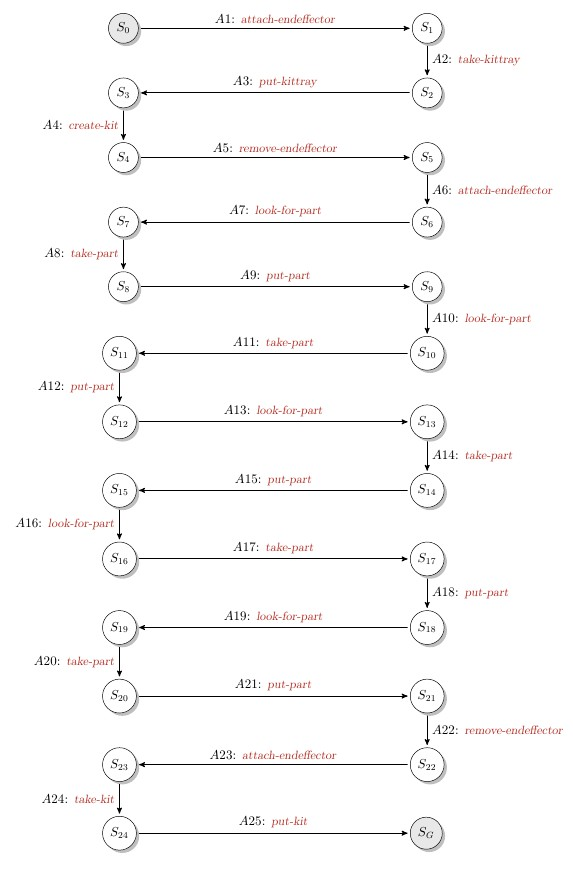
\includegraphics[width=12cm]{Figure/generated-plan.jpg}
\scalebox{.7}{
\begin{tikzpicture}[node distance=1.5cm, every edge/.style={link}]

  %%%%%%%%%%%%%%%%%%%%%%%%%%%%%%%%%%%%%%%%%%%%
  %---------- Main
  %%%%%%%%%%%%%%%%%%%%%%%%%%%%%%%%%%%%%%%%%%%%
  \node[cloud2] (S0)  {$S_0$};
  \node[cloud] (S1) [right=8cm of S0]{$S_1$};
  \node[cloud] (S2) [below=1cm of S1]{$S_2$};
  \node[cloud] (S3) [left=8cm of S2]{$S_3$};
  \node[cloud] (S4) [below=1cm of S3]{$S_4$};
  \node[cloud] (S5) [right=8cm of S4]{$S_5$};
  \node[cloud] (S6) [below=1cm of S5]{$S_6$};
  \node[cloud] (S7) [left=8cm of S6]{$S_7$};
  \node[cloud] (S8) [below=1cm of S7]{$S_8$};
  \node[cloud] (S9) [right=8cm of S8]{$S_9$};
  \node[cloud] (S10) [below=1cm of S9]{$S_{10}$};
  \node[cloud] (S11) [left=8cm of S10]{$S_{11}$};
  \node[cloud] (S12) [below=1cm of S11]{$S_{12}$};
  \node[cloud] (S13) [right=8cm of S12]{$S_{13}$};
  \node[cloud] (S14) [below=1cm of S13]{$S_{14}$};
  \node[cloud] (S15) [left=8cm of S14]{$S_{15}$};
  \node[cloud] (S16) [below=1cm of S15]{$S_{16}$};
  \node[cloud] (S17) [right=8cm of S16]{$S_{17}$};
  \node[cloud] (S18) [below=1cm of S17]{$S_{18}$};
  \node[cloud] (S19) [left=8cm of S18]{$S_{19}$};
  \node[cloud] (S20) [below=1cm of S19]{$S_{20}$};
  \node[cloud] (S21) [right=8cm of S20]{$S_{21}$};
  \node[cloud] (S22) [below=1cm of S21]{$S_{22}$};
  \node[cloud] (S23) [left=8cm of S22]{$S_{23}$};
  \node[cloud] (S24) [below=1cm of S23]{$S_{24}$};
  \node[cloud2] (SG) [right=8cm of S24]{$S_G$};

\draw[myarrow] (S0.east) -- node [above] {$A1$: \opsmall{attach-endeffector}}(S1.west);
\draw[myarrow] (S1.south) -- node [right] {$A2$: \opsmall{take-kittray}}(S2.north);
\draw[myarrow] (S2.west) --  node [above] {$A3$: \opsmall{put-kittray}}(S3.east);
\draw[myarrow] (S3.south) --  node [left] {$A4$: \opsmall{create-kit}}(S4.north);
\draw[myarrow] (S4.east) --  node [above] {$A5$: \opsmall{remove-endeffector}}(S5.west);
\draw[myarrow] (S5.south) --  node [right] {$A6$: \opsmall{attach-endeffector}}(S6.north);
\draw[myarrow] (S6.west) --  node [above] {$A7$: \opsmall{look-for-part}}(S7.east);
\draw[myarrow] (S7.south) --  node [left] {$A8$: \opsmall{take-part}}(S8.north);
\draw[myarrow] (S8.east) --  node [above] {$A9$: \opsmall{put-part}}(S9.west);
\draw[myarrow] (S9.south) --  node [right] {$A10$: \opsmall{look-for-part}}(S10.north);
\draw[myarrow] (S10.west) --  node [above] {$A11$: \opsmall{take-part}}(S11.east);
\draw[myarrow] (S11.south) --  node [left] {$A12$: \opsmall{put-part}}(S12.north);
\draw[myarrow] (S12.east) --  node [above] {$A13$: \opsmall{look-for-part}}(S13.west);
\draw[myarrow] (S13.south) --  node [right] {$A14$: \opsmall{take-part}}(S14.north);
\draw[myarrow] (S14.west) --  node [above] {$A15$: \opsmall{put-part}}(S15.east);
\draw[myarrow] (S15.south) -- node [left] {$A16$: \opsmall{look-for-part}}(S16.north);
\draw[myarrow] (S16.east) -- node [above] {$A17$: \opsmall{take-part}}(S17.west);
\draw[myarrow] (S17.south) -- node [right] {$A18$: \opsmall{put-part}}(S18.north);
\draw[myarrow] (S18.west) -- node [above] {$A19$: \opsmall{look-for-part}}(S19.east);
\draw[myarrow] (S19.south) -- node [left] {$A20$: \opsmall{take-part}}(S20.north);
\draw[myarrow] (S20.east) -- node [above] {$A21$: \opsmall{put-part}}(S21.west);
\draw[myarrow] (S21.south) -- node [right] {$A22$: \opsmall{remove-endeffector}}(S22.north);
\draw[myarrow] (S22.west) -- node [above] {$A23$: \opsmall{attach-endeffector}}(S23.east);
\draw[myarrow] (S23.south) -- node [left] {$A24$: \opsmall{take-kit}}(S24.north);
\draw[myarrow] (S24.east) -- node [above] {$A25$: \opsmall{put-kit}}(SG.west);

\end{tikzpicture}
}
\caption{Example of plan generated with the kitting domain and problem files.}
\label{fig:plan}
\end{figure} 